\section{Evaluation}
\label{sec:evaluation}

The evaluation answers the three research questions with measurements whose protocols were committed before they ran. Every number below comes from a JSON file in the public repository and is given with the environment it was measured in.

\subsection{Setup}

Two environments were used, and timings come only from the second.

\begin{table*}[t]
\caption{Environments. Timings come only from the physical machine.}
\label{tab:env}
\footnotesize
\begin{tabularx}{\textwidth}{@{}>{\raggedright\arraybackslash}p{0.2\textwidth}LL@{}}
\toprule
Environment & Hardware and software & Used for \\
\midrule
Cloud container & Linux x86\_64; Python 3.13; scikit-learn 1.9.1; Go 1.24.7 & Functional correctness, the credit-scoring case, regeneration of the dissertation's runs, tamper attacks in A--B+, answerability; no timing is reported from it \\
Physical machine & Apple M4 Pro (14 cores), 24\,GB; macOS 26.6.2; Python 3.12.7; APFS & Cost ablation (Section~6.5) \\
Same machine, Docker Desktop 29.8.0 (14 CPUs, 8\,GB) & Hyperledger Fabric 2.5.10 (arm64 images); two organisations, one CA each, one Raft orderer; LevelDB, and CouchDB 3.4.2 for a query run & Anchoring (Section~6.6), configuration C of the tamper experiment, audit question Q12 \\
\bottomrule
\end{tabularx}
\end{table*}


The data are the six canonical scenarios and a three-event serious-incident sequence; the Statlog German Credit dataset (1,000 applicants)~\cite{hofmann1994} for the credit-scoring case; and two streams of the MultiFlow industrial platform~\cite{torres2026}: Muvu (29 events) and Steel\_Industry (35,040 readings, 1,750 events). Protocols, results and figure scripts are archived with a DOI~\cite{artefacts} (see the data availability statement).

\subsection{Functional correctness}

The engine reproduces the dissertation's decisions under the version 2 evidence model. The six canonical scenarios yield one approval, three rejections (precision, fairness, missing approval), one escalation for drift and one recorded audit query, each under the same rule as in version 1. The incident sequence yields two escalations under \path{incident.reportable} and one recorded query, all three supporting Art. 73. Re-executing every decision from its record and the archived policy returns the same decision and \path{rule_id} for all 1,788 regenerated records and all 16 records of the credit case.

The input boundary is pinned by a matrix of 24 malformed or edge-case events: the dissertation's 16, plus 8 for the version 2 fields and the numeric domain of RFC 8785. Each case gets the same outcome in the Python issuer and the Go chaincode. The dissertation's sensitivity analysis over 45 threshold combinations still applies to the decision logic, which version 2 left unchanged: approvals range from 0/6 to 4/6, and the decision profile is stable to $\pm$6.25 \% of the precision threshold. The grids for fairness and drift are too coarse to claim fine stability for those thresholds.

\subsection{Real-data cases}

Table~\ref{tab:runs} summarises the five runs. Every chain verifies and every decision re-executes.

\begin{table*}[t]
\caption{Decisions and verification per run (schema version 2).}
\label{tab:runs}
\footnotesize
\begin{tabularx}{\textwidth}{@{}Lrrrrrrr@{}}
\toprule
Run & Events & Approved & Rejected & Escalated & Recorded & Chain & Re-execution \\
\midrule
Canonical scenarios & 6 & 1 & 3 & 1 & 1 & 6/6 & 6/6 \\
Incident sequence (Art. 73) & 3 & 0 & 0 & 2 & 1 & 3/3 & 3/3 \\
Credit scoring, German Credit & 16 & 11 & 4 & 1 & 0 & 16/16 & 16/16 \\
MultiFlow, Muvu (replay) & 29 & 12 & 0 & 17 & 0 & 29/29 & 29/29 \\
MultiFlow, Steel\_Industry (replay) & 1,750 & 94 & 0 & 1,656 & 0 & 1,750/1,750 & 1,750/1,750 \\
\bottomrule
\end{tabularx}
\end{table*}


\textbf{Credit scoring.} The pipeline emits a record at every stage, each run under its own \path{run_id}: ingestion and split of the dataset, training, validation and, for the second model, two deployment requests and six monitoring batches. The protected attribute (age, under 25 against 25 and over, as in AI Fairness 360~\cite{bellamy2019}) and every threshold were fixed before training. The minimum precision, 0.68, was calibrated on a pilot partition that was then discarded. On the validation set, the unmitigated model reaches precision 0.793 and the model trained with reweighing~\cite{kamiran2012} 0.800, but both show a demographic parity difference of 0.112, above the maximum of 0.10. Both validations are therefore rejected under \path{threshold.fairness}, and so are both deployment requests, before the approval rule is reached. This holds whether or not the request carries a valid signed approval.

Monitoring follows the second model on six batches of 50 test cases, with a subgroup over-sampled at a share rising from 0.30 to 0.95. The Population Stability Index~\cite{siddiqi2006} of the scores rises from 0.042 to 0.930 and crosses the threshold of 0.25 only in the last batch, which escalates under \path{monitoring.drift_alert}. The acceptance checks all pass. The 10 metrics in the ledger are recomputed, identically, from the artefacts in the store, and all 16 artefact digests are recomputed from their \path{off_chain_ref}.

A post hoc analysis over 500 partitions shows how much of this outcome is one draw. The reweighed model passes validation in 44 \% of partitions (95 \% interval 40--48 \%) and the unmitigated one in 26 \% (23--30 \%). The decision taken on the validation set agrees with the one the test set would give in only 49 \% and 58 \% of partitions. The evidence records exactly what was decided and on which numbers. The stability of the estimate behind the decision is another matter (Section~7.1).

\textbf{MultiFlow.} The two industrial streams were regenerated under version 2 by replaying the platform's CSV files through the bridge's own logic, without Kafka. Batch by batch, the replay reproduces the dissertation's live runs: the same decision and the same reason, drift score included, for 29 of 29 and 1,750 of 1,750 batches. Only the observational half of the policy is exercised. Precision and parity come from the observer's configuration (0.85 and 0.03), and the approval flag is an assumption, so the escalations measure drift and nothing else.

\subsection{Tamper evidence}

Table~\ref{tab:tamper} gives the observed outcome of each attack on the credit-scoring ledger (16 records; the attacked record is the eighth). In B+ the signed head is published every five records, and in C every record is anchored on the Fabric network. All 48 cells of A--B+ and all nine attacks in C came out as the protocol expected.

\begin{table*}[t]
\caption{Attacks detected by a third party's check, per configuration (observed). In B+ the signed head is published every five records; in C every record is anchored on the Fabric network.}
\label{tab:tamper}
\footnotesize
\begin{tabularx}{\textwidth}{@{}Lccccc@{}}
\toprule
Attack & A & B0 & B & B+ & C \\
\midrule
T1 Alter a field of an intermediate record & no & yes & yes & yes & yes \\
T2 Alter only the signature & -- & -- & yes & yes & yes \\
T3 Alter and recompute every hash, without the key & no & no & yes & yes & yes \\
T4 Swap two records & no & yes & yes & yes & yes \\
T5 Delete an intermediate record & no & yes & yes & yes & yes \\
T6a Truncate a suffix that crosses an anchor & no & no & no & yes & yes \\
T6b Truncate a suffix after the last anchor & no & no & no & no & yes$^{a}$ \\
T7a Rewrite with the issuer's key, crossing an anchor & no & no & no & yes & yes \\
T7b Rewrite with the issuer's key, after the last anchor & no & no & no & no & yes$^{a}$ \\
T8 Omit an event at the source & no & no & no & no & --$^{b}$ \\
T9a Inject a forged event upstream & no & no & no & no & --$^{b}$ \\
T9b Inject a forged approval upstream & no$^{c}$ & no$^{c}$ & no$^{c}$ & no$^{c}$ & --$^{b}$ \\
\bottomrule
\end{tabularx}

\smallskip
\raggedright\footnotesize
$^{a}$ The same records are altered as in B+; in C they are anchored, so no unanchored suffix exists.
$^{b}$ These attacks act before anything reaches a ledger and were not repeated for C.
$^{c}$ The record is well formed and passes the check, but the engine rejects the forged approval at the gate (\path{oversight.approval_invalid}) in every configuration.
-- under A and B0 for T2: no signature to alter.
\end{table*}



T3 measures what the signature adds to the hash chain: without the key, a consistent rewrite of the hashes passes B0 and fails B. T6 and T7 measure what an external anchor adds to a signed log. Truncation and a rewrite by a key holder become detectable, but only up to the last anchor, and anchoring every record on the network closes that window. T8 and T9a are outside the reach of every configuration, because the evidence can only attest what the engine was given. T9b, the one upstream forgery that is caught, is stopped by the engine's check of the approver's signature before anything is stored.

\subsection{Cost of verifiable evidence}

Signing costs little. Table~\ref{tab:cost} gives the latency per event of each arm of the ablation, measured on the physical machine in ten rounds of 200 events after 50 discarded, with the order of the arms rotated by a Williams design.

\begin{table*}[t]
\caption{Latency per event (ms) on the physical machine: median of round medians [IQR over 2,000 events] and 95th percentile. W1: the dissertation's approved validation event; W2: the six canonical scenarios in turn.}
\label{tab:cost}
\footnotesize
\begin{tabularx}{\textwidth}{@{}Lcccc@{}}
\toprule
Arm or paired difference & W1 median [IQR] & W1 P95 & W2 median [IQR] & W2 P95 \\
\midrule
A, SQLite row & 0.26 [0.24 to 0.31] & 0.50 & 0.29 [0.26 to 0.32] & 0.45 \\
B0, hash chain & 0.31 [0.29 to 0.35] & 0.44 & 0.33 [0.30 to 0.37] & 0.52 \\
B, signed & 0.33 [0.30 to 0.37] & 0.48 & 0.34 [0.31 to 0.39] & 0.52 \\
B+, anchored every 100 events & 0.34 [0.31 to 0.38] & 0.46 & 0.35 [0.32 to 0.40] & 0.52 \\
\midrule
B0 $-$ A: canonical form, hashing, append-only file & 0.048 [0.0015 to 0.082] & 0.14 & 0.045 [0.011 to 0.079] & 0.15 \\
B $-$ B0: Ed25519 signature & 0.017 [$-$0.016 to 0.053] & 0.11 & 0.016 [$-$0.019 to 0.052] & 0.12 \\
B $-$ A: verifiable log against a database row & 0.068 [0.022 to 0.098] & 0.16 & 0.059 [0.026 to 0.096] & 0.16 \\
B+ $-$ B: anchoring & 0.0069 [$-$0.027 to 0.039] & 0.099 & 0.0088 [$-$0.027 to 0.043] & 0.12 \\
\bottomrule
\end{tabularx}
\end{table*}


An event takes about 0.3 ms in every arm, the engine's decision included, which all arms share. A verifiable centralised log adds 0.068 ms per event to a plain database row (W1), and the Ed25519 signature accounts for 0.017 ms of that. Anchoring falls on one event in a hundred: the anchor operation itself takes 0.080 ms, and its amortised cost (the mean of B+ $-$ B, $-$0.001 ms) cannot be told apart from zero. On macOS, \path{fsync} does not force the drive's write cache, for the append-only file or for SQLite, so both arms are treated alike.

The cost does not grow with the ledger (Figure~\ref{fig:growth}). Over 10,000 records, the median per block of 1,000 moves from 0.31 to 0.32 ms for B and from 0.27 to 0.26 ms for A, and every arm's ledger verifies at the end. The dissertation's prototype rewrote the whole ledger file on each event, so its latency grew with the ledger. Append-only persistence removed that growth.

\begin{figure}[t]
\centering
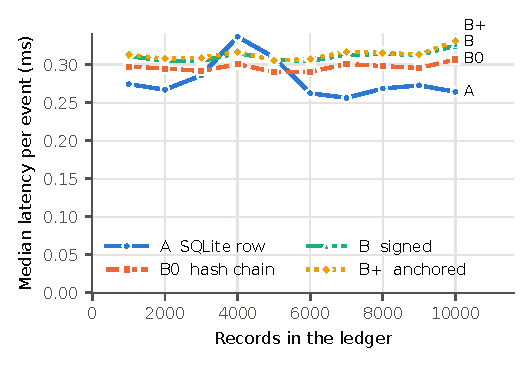
\includegraphics[width=\columnwidth]{figures/F4_latency_vs_ledger_size.pdf}
\caption{Median latency per event against the number of records in the ledger, per arm, in blocks of 1,000 events (W1).}
\label{fig:growth}
\end{figure}

Set against the event cadence of the two real cases, the cost is negligible. At the rate of the live MultiFlow run (21.7 events/s, Section~6.6), a verifiable log adds about 1.5 ms of work per second of stream. The credit-scoring pipeline emits only 16 records over two training runs.

\subsection{Cost of ledger anchoring}

The cost of the ledger lies in ordering. With one transaction in flight, the orderer cuts each block only when its BatchTimeout expires, so every anchoring transaction waits for it, whatever $N$. The latency to durable evidence is 2,028 ms with the 2 s timeout and 278 ms with 250 ms, about 28 ms above the timeout, and it barely moves up to $N=500$ (2,039 and 289 ms; Figure~\ref{fig:anchoring}b). At $N=1$ the network makes 0.49 records durable per second, which reproduces the dissertation's figure of about 0.5.

Throughput therefore grows in proportion to $N$ (Figure~\ref{fig:anchoring}a): from 0.49 to 245 records per second with 2 s, and from 3.6 to 1,730 with 250 ms. An anchor for 500 records is one transaction carrying one Merkle root, so the number of records no longer reaches the network. Backfilling the 1,750 events of the Steel\_Industry stream would take about an hour at $N=1$ with the default timeout, and about one second at $N=500$ with 250 ms.

The price of batching is the wait for a batch to fill. At the event rate of the live MultiFlow run, 21.7 events per second, per-record anchoring cannot keep up with either timeout, and neither can $N=10$ with 2 s: the queue would grow without bound. Where anchoring keeps up, the expected time from emission to durable evidence is the measured anchor latency plus the mean wait to fill the batch, $(N-1)/(2\lambda)$ (Figure~\ref{fig:anchoring}c). It is 0.48 s at $N=10$ with 250 ms, 3.2 s at $N=50$ with 2 s, and 11.8 to 13.6 s at $N=500$. A provider thus chooses $N$ and the timeout from its event rate and from how long a record may stay covered only by its own chain.

\begin{figure*}[t]
\centering
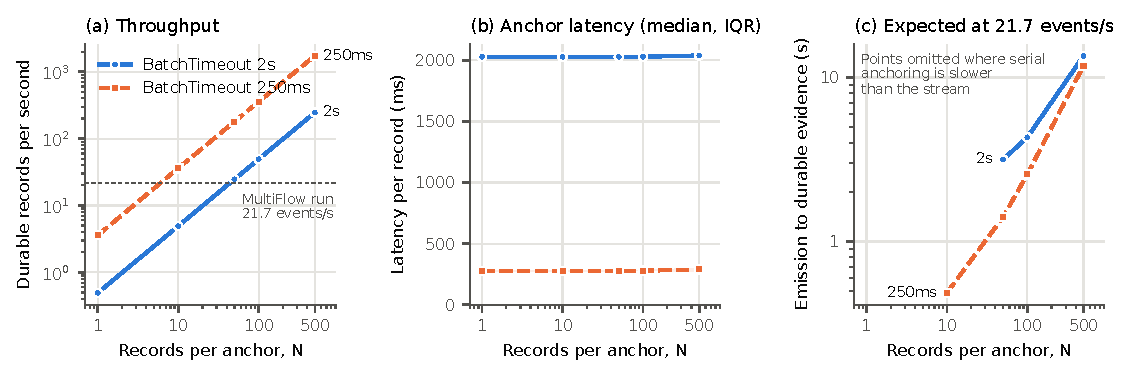
\includegraphics[width=\textwidth]{figures/F5_anchoring_vs_batch_size.pdf}
\caption{Anchoring on the Fabric network against records per anchor, $N$. (a) Durable-evidence throughput, with the event rate of the live MultiFlow run as a reference line. (b) Measured latency per record (median and IQR). (c) Expected time from emission to durable evidence at that rate: the measured latency plus the analytic wait to fill the batch. Points where serial anchoring is slower than the stream are omitted.}
\label{fig:anchoring}
\end{figure*}

Verification is cheap and independent of $N$. \path{VerifyInclusion} takes 1.6 ms (median; 95th percentile 2.3 to 3.1 ms) on both state databases, and an inclusion proof grows with $\log_2 N$, from 337 bytes at $N=10$ to 673 at $N=500$. \path{VerifyChain} over the per-record chain takes 206 ms for 601 records on LevelDB (0.34 ms per record) and 102 ms for 201 records on CouchDB (0.51 ms per record). The CouchDB network held one repetition of the chain against three on LevelDB, so only the per-record figures compare. The first call of each query paid a warm-up of several seconds, which raises the 95th percentile of \path{VerifyChain} in the 2 s run to 438 ms.

The endorsement policy held. An anchor endorsed by Org1 alone was refused at validation with \path{ENDORSEMENT_POLICY_FAILURE} on all three networks. The transaction stays in its block, marked invalid, and the world state did not change.

\subsection{Auditability}

Table~\ref{tab:audit} condenses the answers to the fourteen audit questions of Section~3 in four configurations. In C, the network is represented by a signed log anchored after every record, as the Fabric run provides, and Q12 is answered from the Fabric run itself. The full matrix is in the supplementary material.

\begin{table}[t]
\caption{Audit questions per configuration: number asked (Q), answerable yes / partial / no (Y/P/N), and answers verifiable by a third party (V). Q14, a check that the redacted export discloses nothing it should withhold, applies only to D.}
\label{tab:audit}
\footnotesize
\begin{tabularx}{\columnwidth}{@{}Lccc@{}}
\toprule
Configuration & Q & Y/P/N & V \\
\midrule
A, plain SQLite log & 13 & 3/2/8 & 0 \\
B, signed log, policy archive, artefact store & 13 & 10/2/1 & 6 (+6 in part) \\
C, B anchored on the ledger, complete OSCAL export & 13 & 13/0/0 & 13 \\
D, redacted OSCAL export only & 14 & 3/5/6 & 0 \\
\bottomrule
\end{tabularx}
\end{table}


Q14, a check that the redacted export discloses nothing it should withhold, applies only to D.

C answers every question, and every answer can be checked without trusting the provider. The chaincode stamps the submitting organisation on each anchor, which answers Q12 (Org1MSP for all 16 records). Q2, who approved the deployment, is answerable only where approvals are signed, while A holds a Boolean flag. Q6, whether re-execution reproduces a decision, needs the decision inputs and the policy archive, which only B and C keep. Q11, whether the sequence is complete between two dates, is answerable only in C, because a signed log cannot show that nothing was cut after its last record.

The redacted export answers less, by design. From D alone, Q13 (which articles are supported, with which technical outcome) is answerable but not verifiable, since the export carries anchors and no record bodies. For Q14, none of the 60 items checked appears in the redacted export: artefact names and digests, the subject identifiers derived from them, reasons, metric values, scenario names, and the policy's threshold fields and values. The search of Section~5.5 tried all 356,400 candidate policies against the policy commitment and recovered nothing. The same search on the first version of the export, which carried the plain digest, recovered the policy. With the provider's key, the commitment opened against the archived policy.

\subsection{Interoperability and conformance}
\label{sec:eval-interop}

The evidence crosses three implementations with the same bytes. Every OSCAL export validates against the NIST schema: the complete and redacted exports of the credit case and of the four regenerated runs, and the dissertation's 18 published exports. The Python issuer and the Go chaincode agree on 6 of 6 canonicalisation vectors of version 1 and 4 of 4 of RFC 8785, on the 24 boundary cases, and on the Merkle roots, inclusion proofs and signed anchors of the batched mode. The browser-based Ledger Explorer recomputes the hash of every record of the version 1 and version 2 ledgers.

That agreement was not there at first. Table~\ref{tab:defects} lists the eight defects that appeared between the Python issuer and the Go chaincode, during the dissertation and its later review.

\begin{table*}[t]
\caption{Defects between the Python issuer and the Go chaincode, and their corrections.}
\label{tab:defects}
\footnotesize
\begin{tabularx}{\textwidth}{@{}>{\raggedright\arraybackslash}p{0.16\textwidth}>{\raggedright\arraybackslash}p{0.2\textwidth}LL@{}}
\toprule
Defect & Symptom & Cause & Correction \\
\midrule
HTML and non-ASCII escaping & \path{record_hash} differs between issuer and chaincode & Go's encoder escapes HTML characters and keeps non-ASCII literal; Python's default does the opposite & One canonical form specified on bytes; RFC 8785 in version 2 \\
Fingerprint taken for the key & Every Ed25519 verification fails & The key's SHA-256 fingerprint used as verification material & Key resolved from a registry by its fingerprint \\
Range-read order & Chain reconstruction breaks & Fabric range reads order keys lexicographically, not by insertion & Zero-padded sequence keys \\
\path{0.0} rewritten as \path{0} & Digest diverges by one byte & A float64 round trip in Go drops the issuer's literal & Original number literals kept (\path{json.RawMessage}) \\
Null optional field & A record that verifies at the source fails at the destination & Go decodes null into an empty string & Optional field as a pointer \\
New fields dropped & No record of the new format verifies & \path{encoding/json} silently discards fields the struct does not declare & In version 2, the hash is computed over the record's own members \\
Lone Unicode surrogate & A body signed and verified in Python diverges in Go & Such strings are outside interoperable JSON (RFC 8259, \S8.2) & Input domain restricted to Unicode scalar values \\
Colliding non-text keys & Two different malformed inputs get the same payload digest & An integer key renders like the string of its digits & Normalisation falls back to an ordered list of pairs on collision \\
\bottomrule
\end{tabularx}
\end{table*}


A canonical form must therefore be specified on bytes, independently of any one language's data model, and a shared boundary matrix works as a conformance test between implementations.
